%!TEX program = xelatex
\documentclass[11pt,utf8]{report}
\usepackage[no-math,cm-default]{fontspec}
\usepackage{amsmath}
\usepackage{amsthm}
\usepackage{amssymb}
%\usepackage{xeCJK}
\usepackage{verbatim}
\usepackage{indentfirst}
\usepackage{syntonly}
\usepackage{fancyhdr}
\usepackage[dvipsnames]{xcolor}
\usepackage{graphicx}
\usepackage[top = 1.2in, bottom = 1.2in, left = 1.3in, right = 1.3in]{geometry}
\usepackage{paralist}
\usepackage{ulem}
\usepackage{titlesec}
\usepackage{zhspacing}
\usepackage{booktabs}
\usepackage{multirow}
\usepackage{multicol}
\usepackage{supertabular}
\usepackage{zhspacing}
\usepackage{float}
\usepackage{pdfpages}

\defaultfontfeatures{Mapping=tex-text}
\zhspacing
%\setromanfont{Times New Roman}
\newfontfamily{\zhfont}[BoldFont=Adobe Heiti Std, ItalicFont=Adobe Kaiti Std]{Adobe Song Std}
\setmonofont[Scale=1]{Courier}

\usepackage{array}
\usepackage[unicode=true, colorlinks=true, linkcolor=black, anchorcolor=black, citecolor=black, urlcolor=black]{hyperref}

\begin{document}

\newcommand{\hlink}[1]{\setcounter{footnote}{1}\footnote{\href{#1}{\textsl{\underline{#1}}}}}
\renewenvironment{proof}{\noindent{\textbf{证明:}}}{\hfill $\square$ \vskip 4mm}
\newtheorem{conclusion*}{结论}
\newcommand{\conclusion}[1]{
	\begin{conclusion*}\textup{#1}\end{conclusion*}
}

\let\enumerate\compactenum
\let\endenumerate\endcompactenum
\let\itemize\compactitem
\let\enditemize\endcompactitem
\setlength{\pltopsep}{5pt}
\setlength{\parindent}{2em}
\setlength{\footskip}{30pt}
\setlength{\baselineskip}{1.3\baselineskip}
\renewcommand\arraystretch{1.2}

\pagestyle{fancy}
\renewcommand{\contentsname}{目录}
\renewcommand{\chaptermark}[1]{\markright{第\thechapter 部分 #1}}
%\renewcommand{\sectionmark}[1]{\markright{\thesection.\ #1}}
\renewcommand{\sectionmark}[1]{}
\renewcommand{\subsectionmark}[1]{}
\renewcommand{\figurename}{图}
\renewcommand{\tablename}{表}
\fancyhead[L]{\small THCO MIPS16e\hspace{1em}计算机系统设计与实现报告}
\fancyhead[R]{\small\nouppercase{\rightmark}}
\fancypagestyle{plain}{\fancyhead{}\fancyfoot{}\renewcommand{\headrulewidth}{0pt}}
\renewcommand{\thefootnote}{\fnsymbol{footnote}}

\titleformat{\chapter} % command
[display] % shape
{\bfseries\Large} % format
{\centering\vspace{-4em}第\thechapter 部分} % label
{0ex} % sep
{\rule{\textwidth}{1pt}
\centering\huge} % before-code
[\vspace{-1ex}\rule{\textwidth}{1pt}] % after-code

\newcolumntype{"}{!{\vrule width 1.2pt}}

\setcounter{secnumdepth}{3}

\thispagestyle{plain}

% \pillar:使用一种统一的方法提高行高
\newcommand{\pillar}{ {\Huge \phantom{A}} }

\begin{titlepage}
% 首行的位置往上调整。但vspace前面需要有东西才会起效。
\phantom{Start!}
\vspace{-1.7cm}
\begin{flushleft}
\textit{\Large 清华大学}\\[0.2cm]
\textit{\Large 计算机组成原理}\\[4.2cm]
% Title
{ \fontsize{29}{\baselineskip} \bfseries THCO MIPS16e}\\[0.5cm]
{ \fontsize{27}{\baselineskip} \bfseries 计算机系统设计与实现}\\[0.5cm]
{ \fontsize{25}{\baselineskip} \bfseries 报告}
\end{flushleft}

\vfill
\begin{flushright}
{\large\begin{tabular}{lccc}
\pillar & \multicolumn{3}{c}{\textbf{作者}} \\ 
\cline{2-4}\pillar & 计XX & XXX & 201XXXXXXX \\\pillar & 计XX & XXX & 201XXXXXXX \\
\end{tabular}}
\end{flushright}

\end{titlepage}

\setcounter{tocdepth}{2}
%\renewcommand{\contentsname}{\LARGE 目录}
\tableofcontents
\newpage
\pagenumbering{arabic}
%\setcounter{chapter}{-1}

%\hypersetup{linkcolor = RoyalBlue}

\chapter{概述}

\section{系统概要}

整体上,我们实现了一个支持中断与异常、五级流水线、兼容THCO MIPS16e指令集架构的计算机系统。

具体而言,在硬件方面,我们的计算机系统具有如下特性:
\begin{itemize}
\item \textbf{处理器} 最高可以运行在40MHz,最高可达40MIPS,CPI=1.01。字长16位。
\item \textbf{内存} 按字编址,每个字的宽度为16位。由于16位地址总线宽度限制,内存寻址只支持64K字,即128KiB。
\item \textbf{显示控制器} 支持640x480 @ 60Hz(工业标准)的VGA信号输出,可以显示80x30个ASCII字符,每个字符支持4种前景色和4种背景色组合。
\item \textbf{PS/2接口} 该接口可以配合驱动程序来支持PS/2键盘和鼠标。
\item \textbf{SD卡存储} 这一次,我们突破了以往对于SD卡使用的限制,成功实现了用市面流行的SDHC储存卡存储数据的功能,存储的数据量远远大于板载的Flash,并且SD卡易于更换。此外,SD卡控制器支持DMA,减轻处理器压力。
\item \textbf{GPIO} 结合驱动程序,可以实现SPI总线协议、$I^2C$总线协议、软件串口和点亮数码管等功能,扩展性较好。
\end{itemize}

在软件方面,我们的计算机系统有如下软件设施:
\begin{itemize}
\item \textbf{汇编器} 实验材料中提供的汇编器不易于使用,我们用Python 3重新实现了一个。支持伪指令(如la以及li)的处理,以及立即数大小检查和报错。
\item \textbf{PS/2键盘驱动} 目前,我们只实现了PS/2键盘的驱动程序。驱动程序能够接收键盘发来的数据,并识别通码和断码,转换为ASCII码。
\item \textbf{shell} 支持从键盘读取命令然后调用相应的代码段。
\item \textbf{2048小游戏} 通过字符画的形式实现了一个类似于2048的小游戏,支持保存和加载游戏局面。
\item \textbf{BadApple!!动画播放} 通过读取SD卡中存储的每一帧图像信息并显示到屏幕来播放动画,用来验证SD卡和显示控制器的功能。
\item \textbf{弹幕} 支持在播放动画的时候显示弹幕,用时钟中断实现,用来验证处理器的中断和异常功能是否实现正确。
\item \textbf{内存转储} 支持将内存转储到SD卡,进行进一步的debug工作,也用来验证SD卡的写入功能。
\item \textbf{上电自检程序} 开机的时候会被首先执行,主要用来检测内存是否有错误,或者系统时钟频率是否过高(导致内存访问出错)。检测出错误后会在数码管上显示错误码并在屏幕上(如果显示控制器此时工作正常)显示错误信息和红色[FAIL]字样,然后停机。
\end{itemize}

\section{组内分工}
组内二人的分工如下:
\begin{multicols}{2}
\subsubsection*{谭闻德}
\begin{itemize}
	\item 整体数据通路的绘制
	\item 完整流水线搭建
	\item 前期系统仿真
	\item Store After Load优化的构思
	\item 内部总线设计
	\item GPIO控制器设计与实现
	\item 显示控制器设计与实现
	\item SD卡控制器设计与实现
	\item 汇编器的设计与实现
	\item POST(上电自检)程序的汇编实现
	\item PS/2驱动程序的汇编实现
	\item BadApple!!动画播放程序的汇编实现
	\item shell的汇编实现
	\item 系统集成、调试与测试
	\item 整体文档的撰写
\end{itemize}
\columnbreak
\subsubsection*{刘明华}
\begin{itemize}
	\item 整体数据通路的绘制
	\item 控制信号表的总结
	\item 指令译码模块的实现
	\item Store After Load优化的实现
	\item 显示控制器的实现
	\item PS/2控制器设计与实现
	\item PS/2驱动程序、读取和显示字符串函数的汇编实现
	\item 2048游戏的汇编实现
	\item BadApple!!的弹幕程序的汇编实现
	\item 文档的撰写与排版
\end{itemize}
\end{multicols}

\chapter{设计与实现}

\section{总体架构}
	\par 计算机系统是硬件和软件的完美结合,所以我们的系统也包括硬件和软件部分。
	\par 硬件和软件由指令集联系在一起,我们实现的指令有(不含汇编器支持的伪指令):\texttt{addiu}、\texttt{addiu3}、\texttt{addu}、\texttt{subu}、\texttt{addsp}、\texttt{and}、\texttt{or}、\texttt{not}、\texttt{move}、\texttt{b}、\texttt{beqz}、\texttt{bnez}、\texttt{bteqz}、\texttt{cmp}、\texttt{cmpi}、\texttt{jr}、\texttt{li}、\texttt{lw}、\texttt{sw}、\texttt{lw\_sp}、\texttt{sw\_sp}、\texttt{mtsp}、\texttt{mtih}、\texttt{mfih}、\texttt{mtc0}、\texttt{mfc0}、\texttt{mfpc}、\texttt{sll}、\texttt{sra}、\texttt{sllv}、\texttt{srav}以及\texttt{nop}。

\section{硬件部分}

	整体数据通路和架构如图\ref{datapath}所示。

	\begin{figure}[H]
		\centering
		\setlength{\leftskip}{-40pt}
		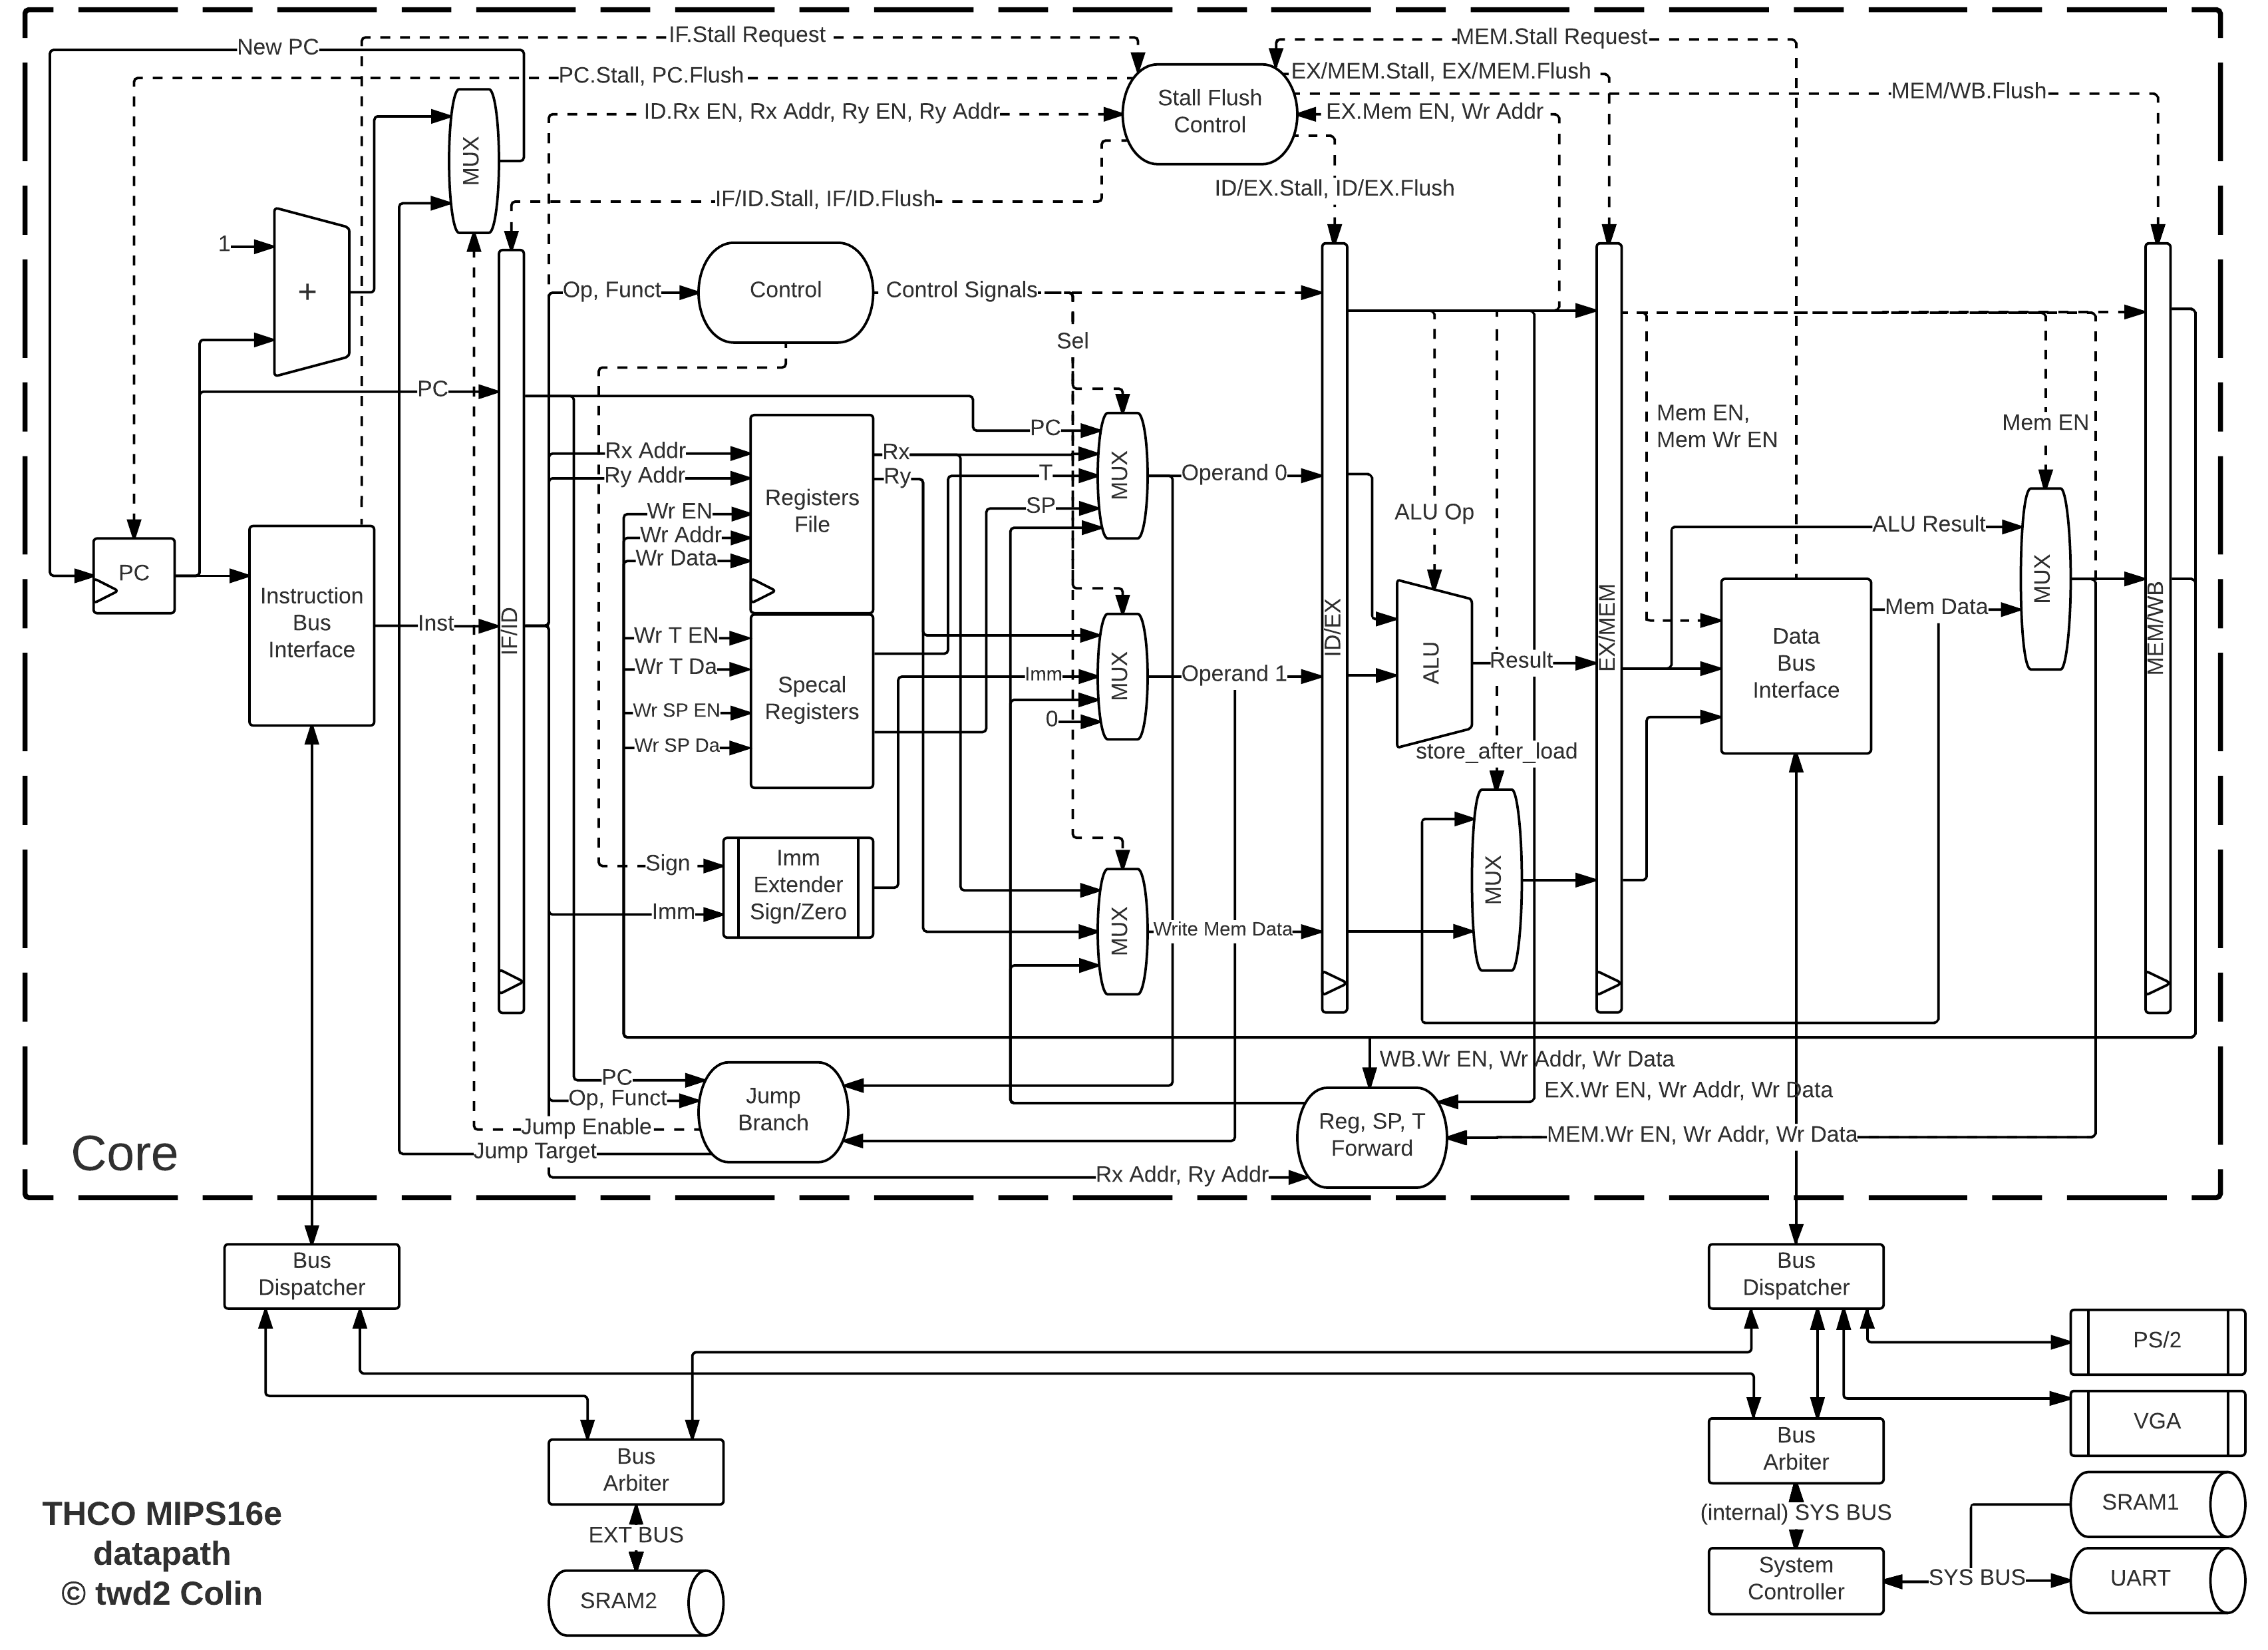
\includegraphics[width=1.2\textwidth]{datapath}
		\caption{数据通路和架构图}
		\label{datapath}
	\end{figure}

\subsection{内部总线设计}
	\par 首先,介绍内部总线设计。内部总线是本系统的最关键的部分,因为它连接了处理器、内存以及其他所有模块,允许模块间相互通信、传输数据。
	\par \textbf{总线分派器}的功能是解析请求方发来的地址,并选择相应的设备,同时实现了IO地址映射。
	\par \textbf{总线仲裁器}的功能是根据某个优先级,确定当前设备处理哪一个请求。我们的实现中,为实现简单,采用固定优先级的做法,优先级为:SD卡控制器DMA请求>处理器访存阶段请求>处理器取指令阶段请求。优先级可能有其他设置,但取指令阶段的请求一定为最低优先级,否则其他部分或全部请求将永远被阻塞。
	\par 实际上,总线分派器和总线仲裁器的本质都是数据选择器,总线分派器选择设备的响应并发给请求方,总线仲裁器选择请求并发送给接在总线上的设备。
	\par 总线分派器和总线仲裁器组合使用,可以灵活地组成各种结构,我们本次实现将处理器、内存和其他外设组成了交叉互联的结构,允许它们互相访问。

\subsection{处理器}
	\par 处理器的内部设计在图\ref{datapath}中已经有清晰的体现,处理器对外的接口有外部中断请求线6根、指令总线接口和数据总线接口。指令总线接口和数据总线接口都连接到内部总线。
	
	\par 控制器中的控制信号的设置如图\ref{control}所示。	
	
	\begin{center}
	\begin{figure}[H]
			\centering
			\setlength{\leftskip}{-40pt}
			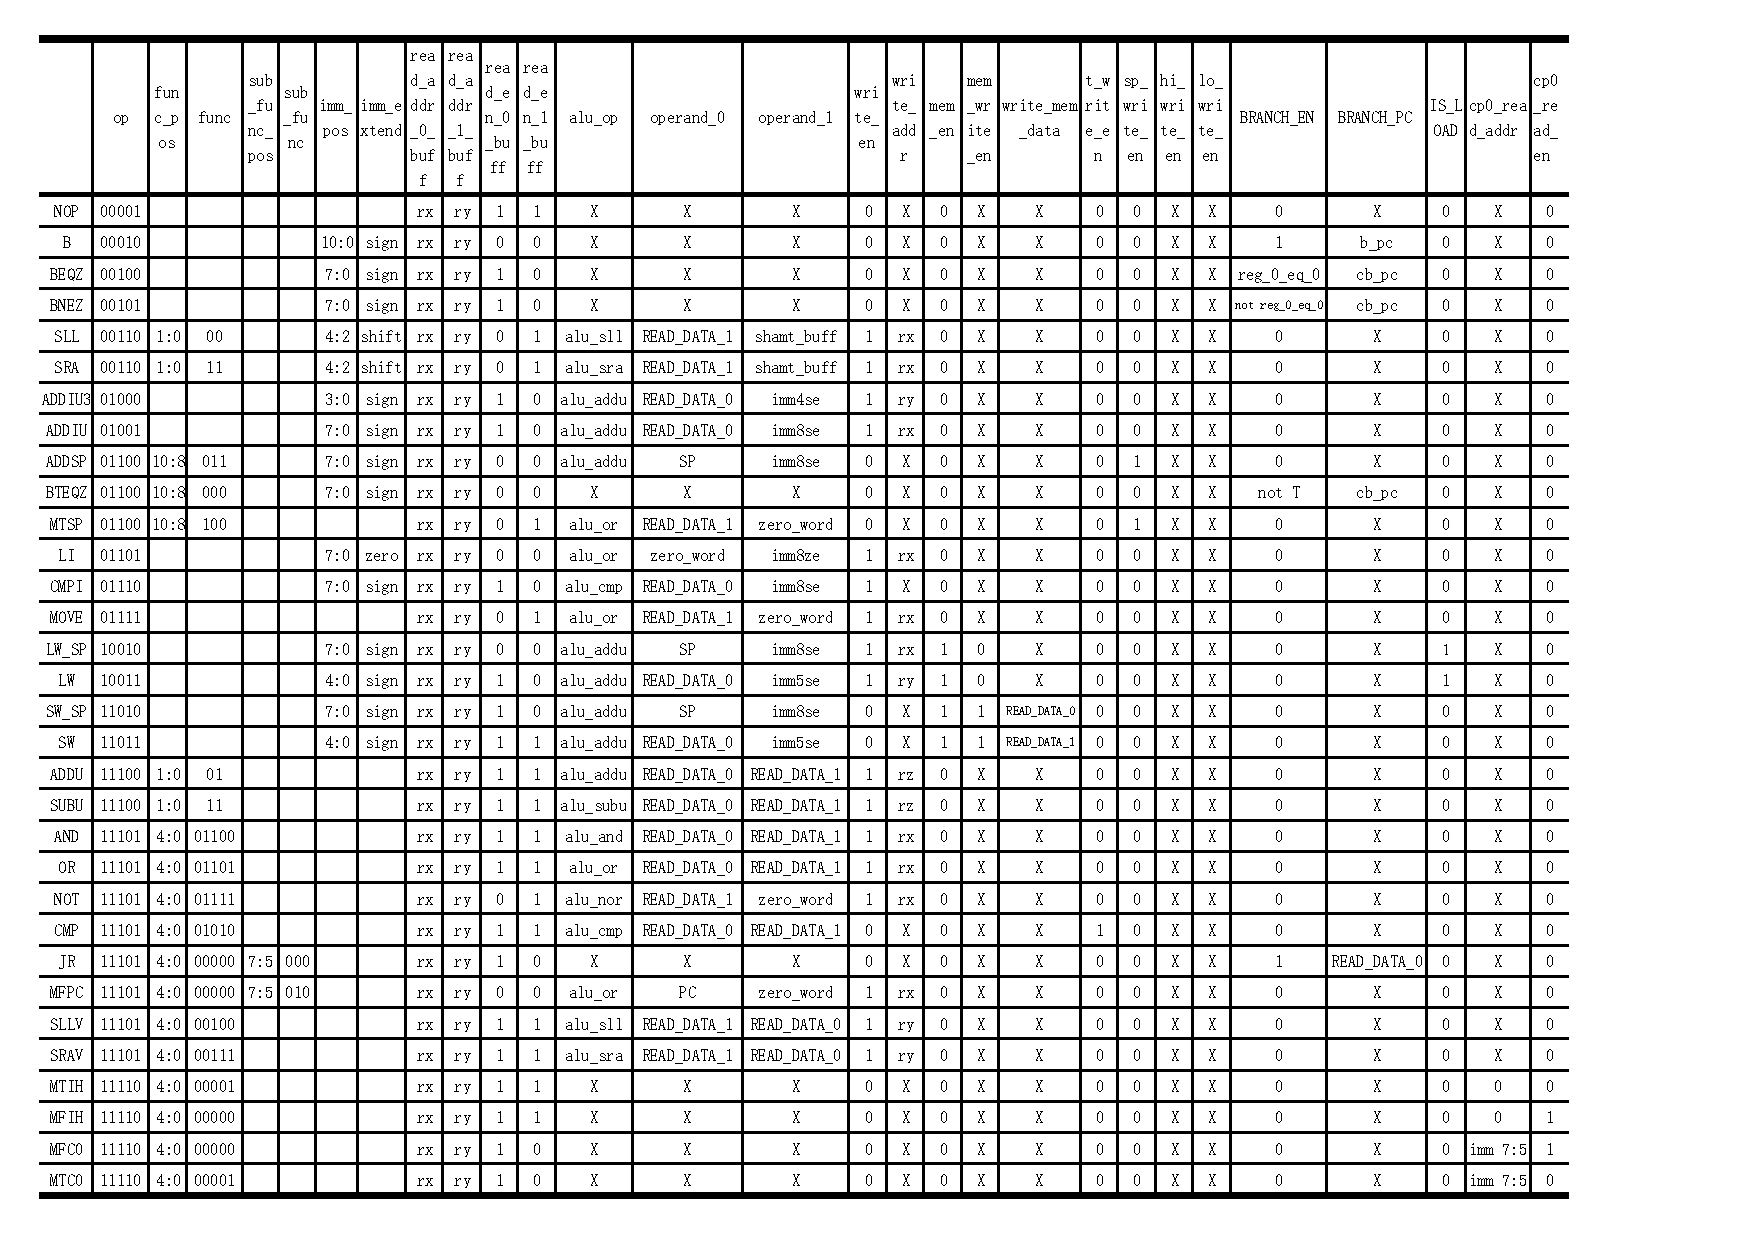
\includegraphics[width=1.2\textwidth]{control.pdf}
			\caption{控制信号表}
			\label{control}
		\end{figure}
	\end{center}

\subsection{SRAM与UART}
	\par 这个模块的作用是将物理总线包装一层,并和内部总线连接,连接在物理总线上面的设备有(处理器片外的)SRAM和(处理器片外的)串口控制器。根据地址的不同,选择不同的设备(SRAM或者串口控制器)访问,SRAM使用\texttt{$\mathtt{\overline{OE}}\mbox{和}\mathtt{\overline{WE}}$}信号控制,串口使用\texttt{wrn}以及\texttt{rdn}信号控制。
	\par 若地址为\texttt{0xBF00},则让串口控制器驱动物理总线,即置\texttt{wrn}或\texttt{rdn}为有效;否则,让SRAM工作,即置\texttt{$\mathtt{\overline{OE}}\mbox{或}\mathtt{\overline{WE}}$}为有效。
	
	\par 此外,串口控制器有\texttt{data\_ready}、\texttt{tbre}以及\texttt{tsre}控制信号,我们把它们映射到地址\texttt{0xBF01}对应的字,作为串口控制寄存器。
	
	\par 从后文可以看出,其他IO都被映射到了\texttt{0xE000}以上的地址,这里把串口控制器的地址映射到\texttt{0xBF00}和\texttt{0xBF01}是出于兼容性的考虑。

\subsection{显示控制器}
	\par TODO。

\subsection{PS/2控制器}
	PS/2控制器主要用于接受PS/2接口传来的信号,将其进行解析后存入缓冲器,同时响应总线发来的读取请求。其中,地址\texttt{0xE003}映射到PS/2控制器的控制寄存器,程序可以通过访问此地址得知当前是否有未读取的新数据;地址\texttt{0xE002}映射到PS/2控制器的数据缓冲寄存器,程序可以通过访问此地址获取最后一次读到的数据。

	显然,PS/2的信号来自于不同的时钟域,也会有跨时钟域的问题。这里,我们对信号用主时钟进行了采样,并通过用触发器延迟两个周期的方法得到采样后的稳定的信号。

	PS/2的信号分为时钟信号和数据信号,我们使用了一个有六个状态的状态机来对PS/2的信号进行处理,依次检测PS/2时钟信号的下降沿并读取其起始位、八个数据位、奇偶校验位和结束位。我们还在每个状态设置了一个计时器,当在一个状态停留过久时,状态机会自动回到初始的等待状态,以避免时钟信号突发错误而带来的状态错乱,提高了PS/2控制器的稳定性。

\subsection{SD卡控制器}
	\par 我们的系统选择SD卡作为外部的块存储设备,所有和SD卡访问相关的电路都实现在这个模块中。这个模块实现的重点在于SD卡的存取。
	
	\par SD卡支持两种接口,SDIO和SPI。其中,SDIO接口比较复杂且封闭,SPI则比较自由且资料相对较多,所以我们主要研究的是通过SPI来存取SD卡中的信息。SD卡分为标准容量的SDSC卡(小于等于2GB)、大容量的SDHC卡(2GB$\sim$32GB)以及更大容量的SDXC卡(32GB$\sim$2TB),我们尝试全部支持。
	
	\par SPI是一种同步串行总线,它根据时钟相位、锁存数据的时机可以分为$2 \times 2=4$种模式。SD卡支持的是模式0,即时钟上升沿锁存数据,下降沿发送数据。此外,SPI收发数据时,\textbf{最高有效位}(\textbf{MSB})先被处理。
	\par SPI使用了四条数据线:
	\begin{itemize}
		\item \texttt{SCLK} 时钟,主机产生
		\item \texttt{$\mathtt{\overline{SS}}\mbox{或}\mathtt{\overline{CS}}$} 从机选择,一般是低有效
		\item \texttt{MOSI或DI} 主机发送,从机接收
		\item \texttt{MISO或DO} 从机发送,主机接收,需要上拉电阻
	\end{itemize}
	
	与SD卡管脚的对应关系如图\ref{sd}\footnote{图片来自\url{http://elm-chan.org/docs/mmc/mmc\_e.html}}所示。
	
	\begin{figure}[h!]
		\centering
		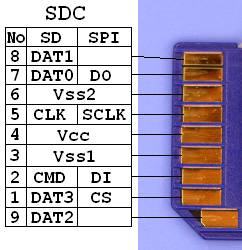
\includegraphics[width=0.3\textwidth]{sd}
		\caption{SD卡接口}
		\label{sd}
	\end{figure}
	
	\par 本次实现中,我们使用状态机来产生SPI总线的时钟、控制信号以及收发数据,为了方便状态机的设计,我们将产生时钟以及发送和接收SPI总线的数据作为了\textbf{子过程}(\textbf{subroutine}),方便其他状态“调用”。
	
	\par 为了访问SD卡中的数据,首先要对SD卡进行上电初始化,图\ref{spi_init}\footnote{图片来自于SD Specifications Part 1 Physical Layer Simplified Specification Version 6.00 Figure 7-2}是SD卡规范中提供的初始化流程,本次实现我们也是严格按照这个流程图实现的,不过虚框中的可选项我们没有实现。该流程图已经十分详细,不过还需要详细说明的是“Power-on”过程、CMD的发送和响应的接收。
	
	\begin{figure}[h!]
		\centering
		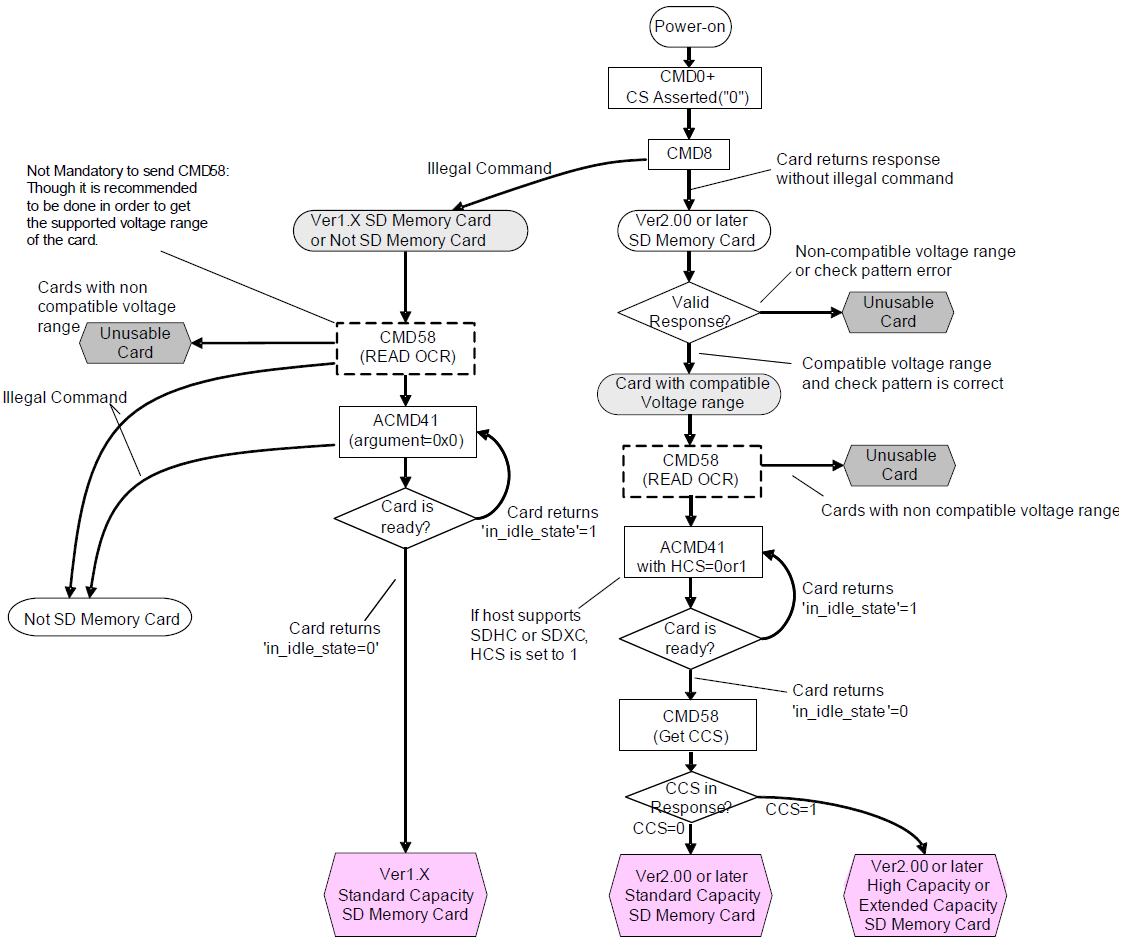
\includegraphics[width=\textwidth]{spi_init}
		\caption{SPI模式初始化流程}
		\label{spi_init}
	\end{figure}
	
	\paragraph{“Power-on”过程} 最开始的上电过程需要等待1ms,等SD卡电压达到所需电压,然后在$\mathtt{\overline{CS}}$拉高的情况下,\texttt{SCLK}产生至少74个时钟周期用于SD卡上电初始化。接着,才可以进行CMD命令的发送。

	\paragraph{CMD的发送} CMD命令长度固定为6个字节,格式如图\ref{cmd}\footnote{图片来自于SD Specifications Part 1 Physical Layer Simplified Specification Version 6.00 Table 7-1},发送时只需要正确构造即可。SPI模式下,SD卡不会验证命令的CRC,但相应的位还需要控制器发送,具体内容随意即可。但是,SD卡接收CMD0命令时还没有进入SPI模式,所以CMD0命令需要设置正确的CRC(硬编码即可);SD卡规范中规定CMD8命令的CRC校验一直打开,故CMD8命令也需要设置正确的CRC(同样,硬编码即可)。本模块用到的命令见表\ref{cmds},命令的编号为十进制数。
	
	\begin{figure}[h!]
		\centering
		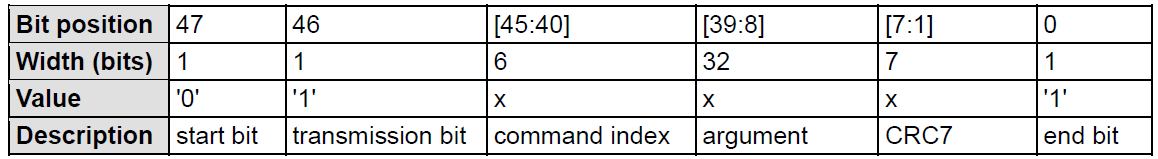
\includegraphics[width=\textwidth]{cmd}
		\caption{CMD命令格式}
		\label{cmd}
	\end{figure}
	
	\begin{table}[h]
	\centering
	\begin{tabular}{c|l}
	\toprule[1.2pt]
	\multicolumn{1}{c|}{\textbf{命令}} & \multicolumn{1}{c}{\textbf{说明}} \\
	\midrule[1.2pt]
	\texttt{CMD0} & 上电初始化 \\ \hline
	\texttt{CMD8} & 检查电压情况 \\ \hline
	\texttt{CMD55} & 所有\texttt{ACMD}的前序命令 \\ \hline
	\texttt{ACMD41} & 进行初始化,获得是否已经初始化好 \\ \hline
	\texttt{CMD58} & 读取OCR(寄存器)内容 \\ \hline
	\texttt{CMD16} & 设置块长度 \\ \hline
	\texttt{CMD17} & 读取单个块 \\ \hline
	\texttt{CMD25} & 写入多个块 \\
	\bottomrule[1.2pt]
	\end{tabular}
	\caption{SD卡命令}
	\label{cmds}
	\end{table}
	
	\paragraph{响应的接收} 在CMD被发送之后,需要等待若干个时钟周期,直到响应到来,表现为\texttt{MISO}被拉低(之前被上拉电阻或SD卡拉高)。然后,即可根据之前发送的CMD类型,接收不同长度的响应数据。本模块使用到的命令对应的响应有三种:1字节的R1、5字节的R3和5字节的R7。一般命令的响应为R1,具体内容如图\ref{r1}\footnote{图片来自于SD Specifications Part 1 Physical Layer Simplified Specification Version 6.00 Figure 7-9}所示。CMD58由于需要返回OCR(Operation Conditions Register)的内容,所以响应为R3;CMD8命令也需要返回额外的信息,所以响应为R7。事实上,R3就是R1后紧随一个OCR字段,R7就是R1后紧随CMD8的响应数据。注意,当SD卡收到了无法识别的命令时,响应一律为R1。
	
	\begin{figure}[h!]
		\centering
		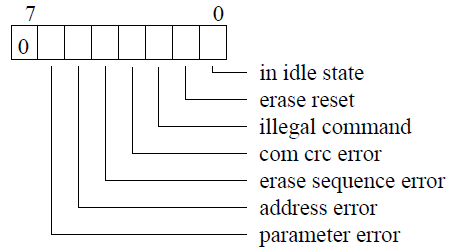
\includegraphics[width=0.5\textwidth]{r1}
		\caption{R1具体内容}
		\label{r1}
	\end{figure}

	\par 成功初始化之后,可以开始进行读写扇区等操作。为了确保每次操作的块恰好是一个扇区(这方便之后的使用),我们在读写操作之前还发送了CMD16命令,设置块大小就为一个扇区的大小,512字节。注意,事实上只有SDSC卡需要这个命令,SDHC或SDXC卡读写操作的块大小固定为512字节。
	
	\par 读扇区使用CMD17命令,参数包含一个地址。值得注意的是,在初始化流程中,如果检测出SD卡为SDSC,则寻址方式为按字节寻址;如果SD卡为SDHC或SDXC,则按照块(或扇区)寻址(从0开始),每块大小512字节,这是在SD卡规范一个表格的注释中说明的\footnote{具体出现在SD Specifications Part 1 Physical Layer Simplified Specification Version 6.00 Table 7-3}。 
	
	\begin{figure}[h!]
		\centering
		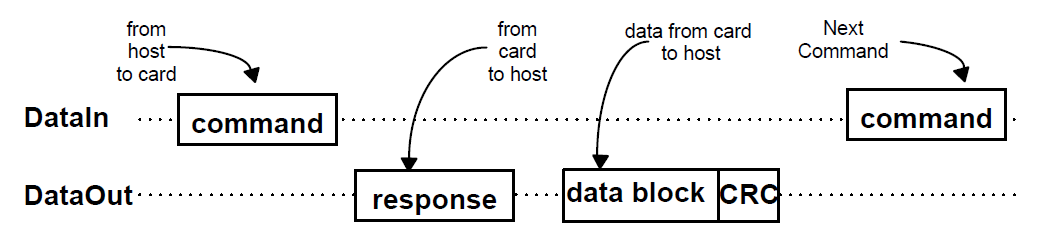
\includegraphics[width=\textwidth]{cmd17}
		\caption{CMD17读扇区流程}
		\label{cmd17}
	\end{figure}
	
	\par 图\ref{cmd17}\footnote{图片来自于SD Specifications Part 1 Physical Layer Simplified Specification Version 6.00 Figure 7-3}清晰地展示了CMD17命令的时序,CMD17命令的响应除了一个字节的R1响应以外,一段时间后还会发送一个data block以及相应的CRC。
	
	\par data block由一个字节的token和后续1$\sim$2048个字节的数据组成。状态机可以检测token来得知data block的到来,token分为两种:数据token(11111110)和错误token(000后跟5位错误码)。当检测到数据token,说明数据正常读取,可以进行接收了;当检测到错误token就要做相应的错误处理,我们的实现是直接停机。两个字节的CRC紧随data block之后,由于SPI模式中没有开启CRC校验,状态机只需要读取这两个字节并丢弃即可。
	
	\par 考虑到优化寄存器资源的使用,我们没有读完一整个扇区再进行内存的写操作,因为那样需要使用512字节的寄存器(共4096位)作为缓冲区。我们的实现中,每读到2个字节就写内存一次,因为内存数据总线宽度为16位,就是2个字节。有一点需要注意,就是\textbf{字节序}的问题,即连续读到的2个字节中哪一个作为内存中一个字的高字节,哪一个作为低字节。我们使用\textbf{小端序},即SD卡低地址的字节,亦即先被读取到的字节,对应内存中一个字更低的字节。
	
	\begin{figure}[h!]
		\centering
		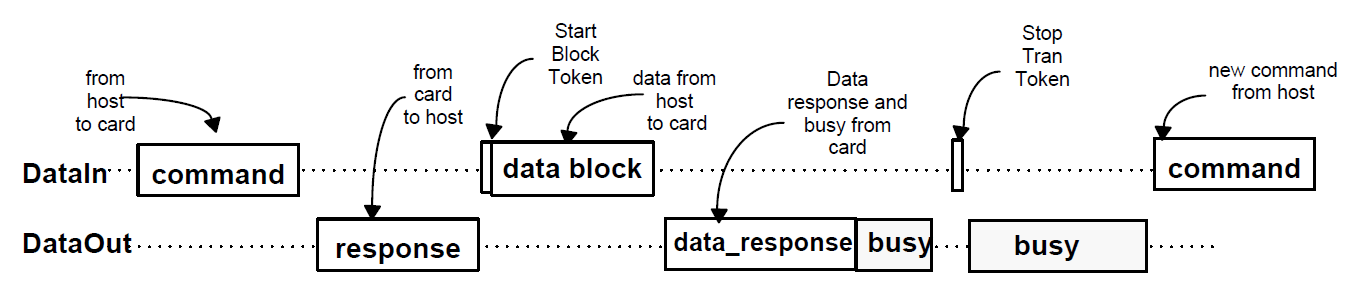
\includegraphics[width=\textwidth]{cmd25}
		\caption{CMD25连续写扇区流程}
		\label{cmd25}
	\end{figure}
	
	\par 对于写入操作而言,我们使用了连续写入命令CMD25来优化写入速度,图\ref{cmd25}\footnote{图片来自于SD Specifications Part 1 Physical Layer Simplified Specification Version 6.00 Figure 7-7}清晰地展示了CMD25命令的时序。这个命令同样包含一个地址参数,寻址方式和读取命令一样,也区分字节寻址以及块(或扇区)寻址。发送命令后需要等待R1响应,若响应正常,发送start block token(实际上就是8个1)后即可开始发送data block来写入。CMD25的data block格式和CMD17的完全类似,区别仅在于发送的时候token取为写入数据token(11111100)。此外,发送data block时CRC字段同样需要发送,但由于SPI模式没有开启CRC校验,所以发送的内容可以任意。每发送一个data block后需要等待一个8位的数据响应,如果响应的后5位为00101则说明数据被接受,之后\texttt{MISO}会被SD卡持续拉低,等到\texttt{MISO}恢复为高则可以继续发送下一个data block。当所有需要写入的data block发送完毕并接收到响应之后,可以发送stop token(11111101 )来停止这次连续写操作。等待8个时钟周期后,\texttt{MISO}会被SD卡持续拉低一段时间,等到\texttt{MISO}恢复为高则说明本次写入操作完成。需要注意的是,执行完CMD25后还应当检查实际写入的块数(因为有些错误无法立刻发现),但本次实现没有考虑。
	
	\par SD卡控制器对处理器的接口表现为几个寄存器:
	\begin{itemize}
		\item \textbf{起始扇区号寄存器} 下一次请求要操作的起始扇区号。
		\item \textbf{内存起始地址寄存器} 下一次请求要操作的起始内存地址。
		\item \textbf{扇区数寄存器} 下一次请求要操作的扇区数。
		\item \textbf{响应寄存器} 这个寄存器目前只有一个中断标志位,表明上次的操作是否已经完成。中断标志位写1清零。
		\item \textbf{请求寄存器} 这个寄存器不是真实存在的寄存器,而是一个端口。向这个寄存器写入数据就相当于给SD卡控制器的状态机发送请求,让其开始执行操作。操作码\texttt{0x0001}为读取操作,\texttt{0x0002}为写入。
	\end{itemize}
	
	\par 本模块整体状态机十分复杂,这里就不展示了。
	
	\par 经过实际测试,本模块确保可以支持这些SD卡:
	
	\begin{itemize}
		\item (SDHC)Kingston 8GB Class 4 Micro SD
		\item (SDHC)Kingston 16GB Class 4 Micro SD
		\item (SDHC)SONY UHS-1 8G Class 10 microSDHC
		\item (SDHC)SONY UHS-1 16G Class 10 microSDHC
		\item (SDSC)某品牌2GB存储卡
		\item (SDSC)SanDisk 1GB Micro SD
	\end{itemize}
	
	\par 遗憾的是,由于不明原因,对于SanDisk某些特定型号的存储卡,无法支持。由于时间和材料限制,我们没有测试SDXC卡,不过SDXC卡与SDHC卡差别不大,理论上也应该能够很好的支持。
	
	\par \textbf{注:}Micro SD卡与普通SD卡区别仅仅在于形状。
	
	\par 本模块可以算是本项目中实现、调试较有挑战性的一部分,我们在参考了互联网大量资料的情况下,利用周末累计调试了两天半(包括休息)才完成。
	\par 此外,由于我们使用了易于其他广泛使用的计算机系统读写和易于替换的SD卡,我们未来可以通过软件实现文件系统的处理,从而更好地支持和其他计算机系统的文件交换。

\subsection{GPIO}
	\par 这个模块就是将FPGA的三态门包装了一层。输出使能接到GPIO控制器的方向寄存器,低有效。输入输出数据接到GPIO的数据寄存器。如此简单的封装,给予了程序直接访问FPGA的IO引脚的能力,能够大大提高灵活性。

\section{软件部分}

\subsection{汇编器}
	\par TODO。
	\par 事实上,一般情况下,汇编成机器码之后还需要进行链接,但是在我们的系统中,链接的工作在汇编前手动完成。
	
\subsection{汇编程序调用约定}
	\par 在编写汇编程序时,我们约定:
	\begin{itemize}
		\item 寄存器r7存放返回地址
		\item 寄存器r0$\sim$r7均由\textbf{被调用者}保存
		\item r0、r1、r2以及r3分别为第一、第二、第三和第四个参数(如果存在),其余参数通过栈传递
		\item 如果有返回值,存放在r4内,此时r4由\textbf{调用者}保存
		\item 全局符号名不以下划线开始,内部符号名以下划线开始,但汇编器不会检查
	\end{itemize}

\subsection{PS/2键盘驱动}
	在本系统中,我们用汇编语言实现了\texttt{getchar}和\texttt{gets}函数,支持同步阻塞地从PS/2键盘读取字符或字符串。

	其中\texttt{getchar}从键盘读入一个扫描码,后通过查表的方式将读取到的键盘扫描码转换为对应字符的ASCII码,并将其存入r4寄存器返回。

	\texttt{gets}则用于从键盘读入一个以换行符结尾的字符串,存入由r0指定的内存地址,并回显到屏幕。其中读入时支持退格。

	具体来说,读入时我们通过r0寄存器得到读取字符串的存储地址,并不断阻塞地从键盘读取字符,若读到的是回退符,则进行相应的回退处理,否则将其查表转换为ASCII码后存入指定内存并进行显示,并在读取到换行符时结束读取。

\subsection{上电自检程序}
	\par TODO。

\subsection{shell}
	\par 我们用实现好的基础函数\texttt{getchar}、\texttt{gets}、\texttt{putchar}以及\texttt{puts}实现了一个类似Unix的简易的shell。shell通过比对字符串是否和已有字符串相等来得知用户想要执行什么命令,然后跳转到相应的代码段。
	\par shell显示时还支持回车、换行和滚屏,这都是由\texttt{putchar}和\texttt{puts}实现的。显示时,我们首先判断当前需要显示的字符是回车、换行还是普通字符,分别对其进行处理,显示完一个字符后再检查是否需要自动换行和滚屏处理。其中,光标的位置和闪烁频率,存放在显示控制器的寄存器中。

\subsection{2048小游戏}
	\begin{center}
	\begin{figure}[H]
			\centering
			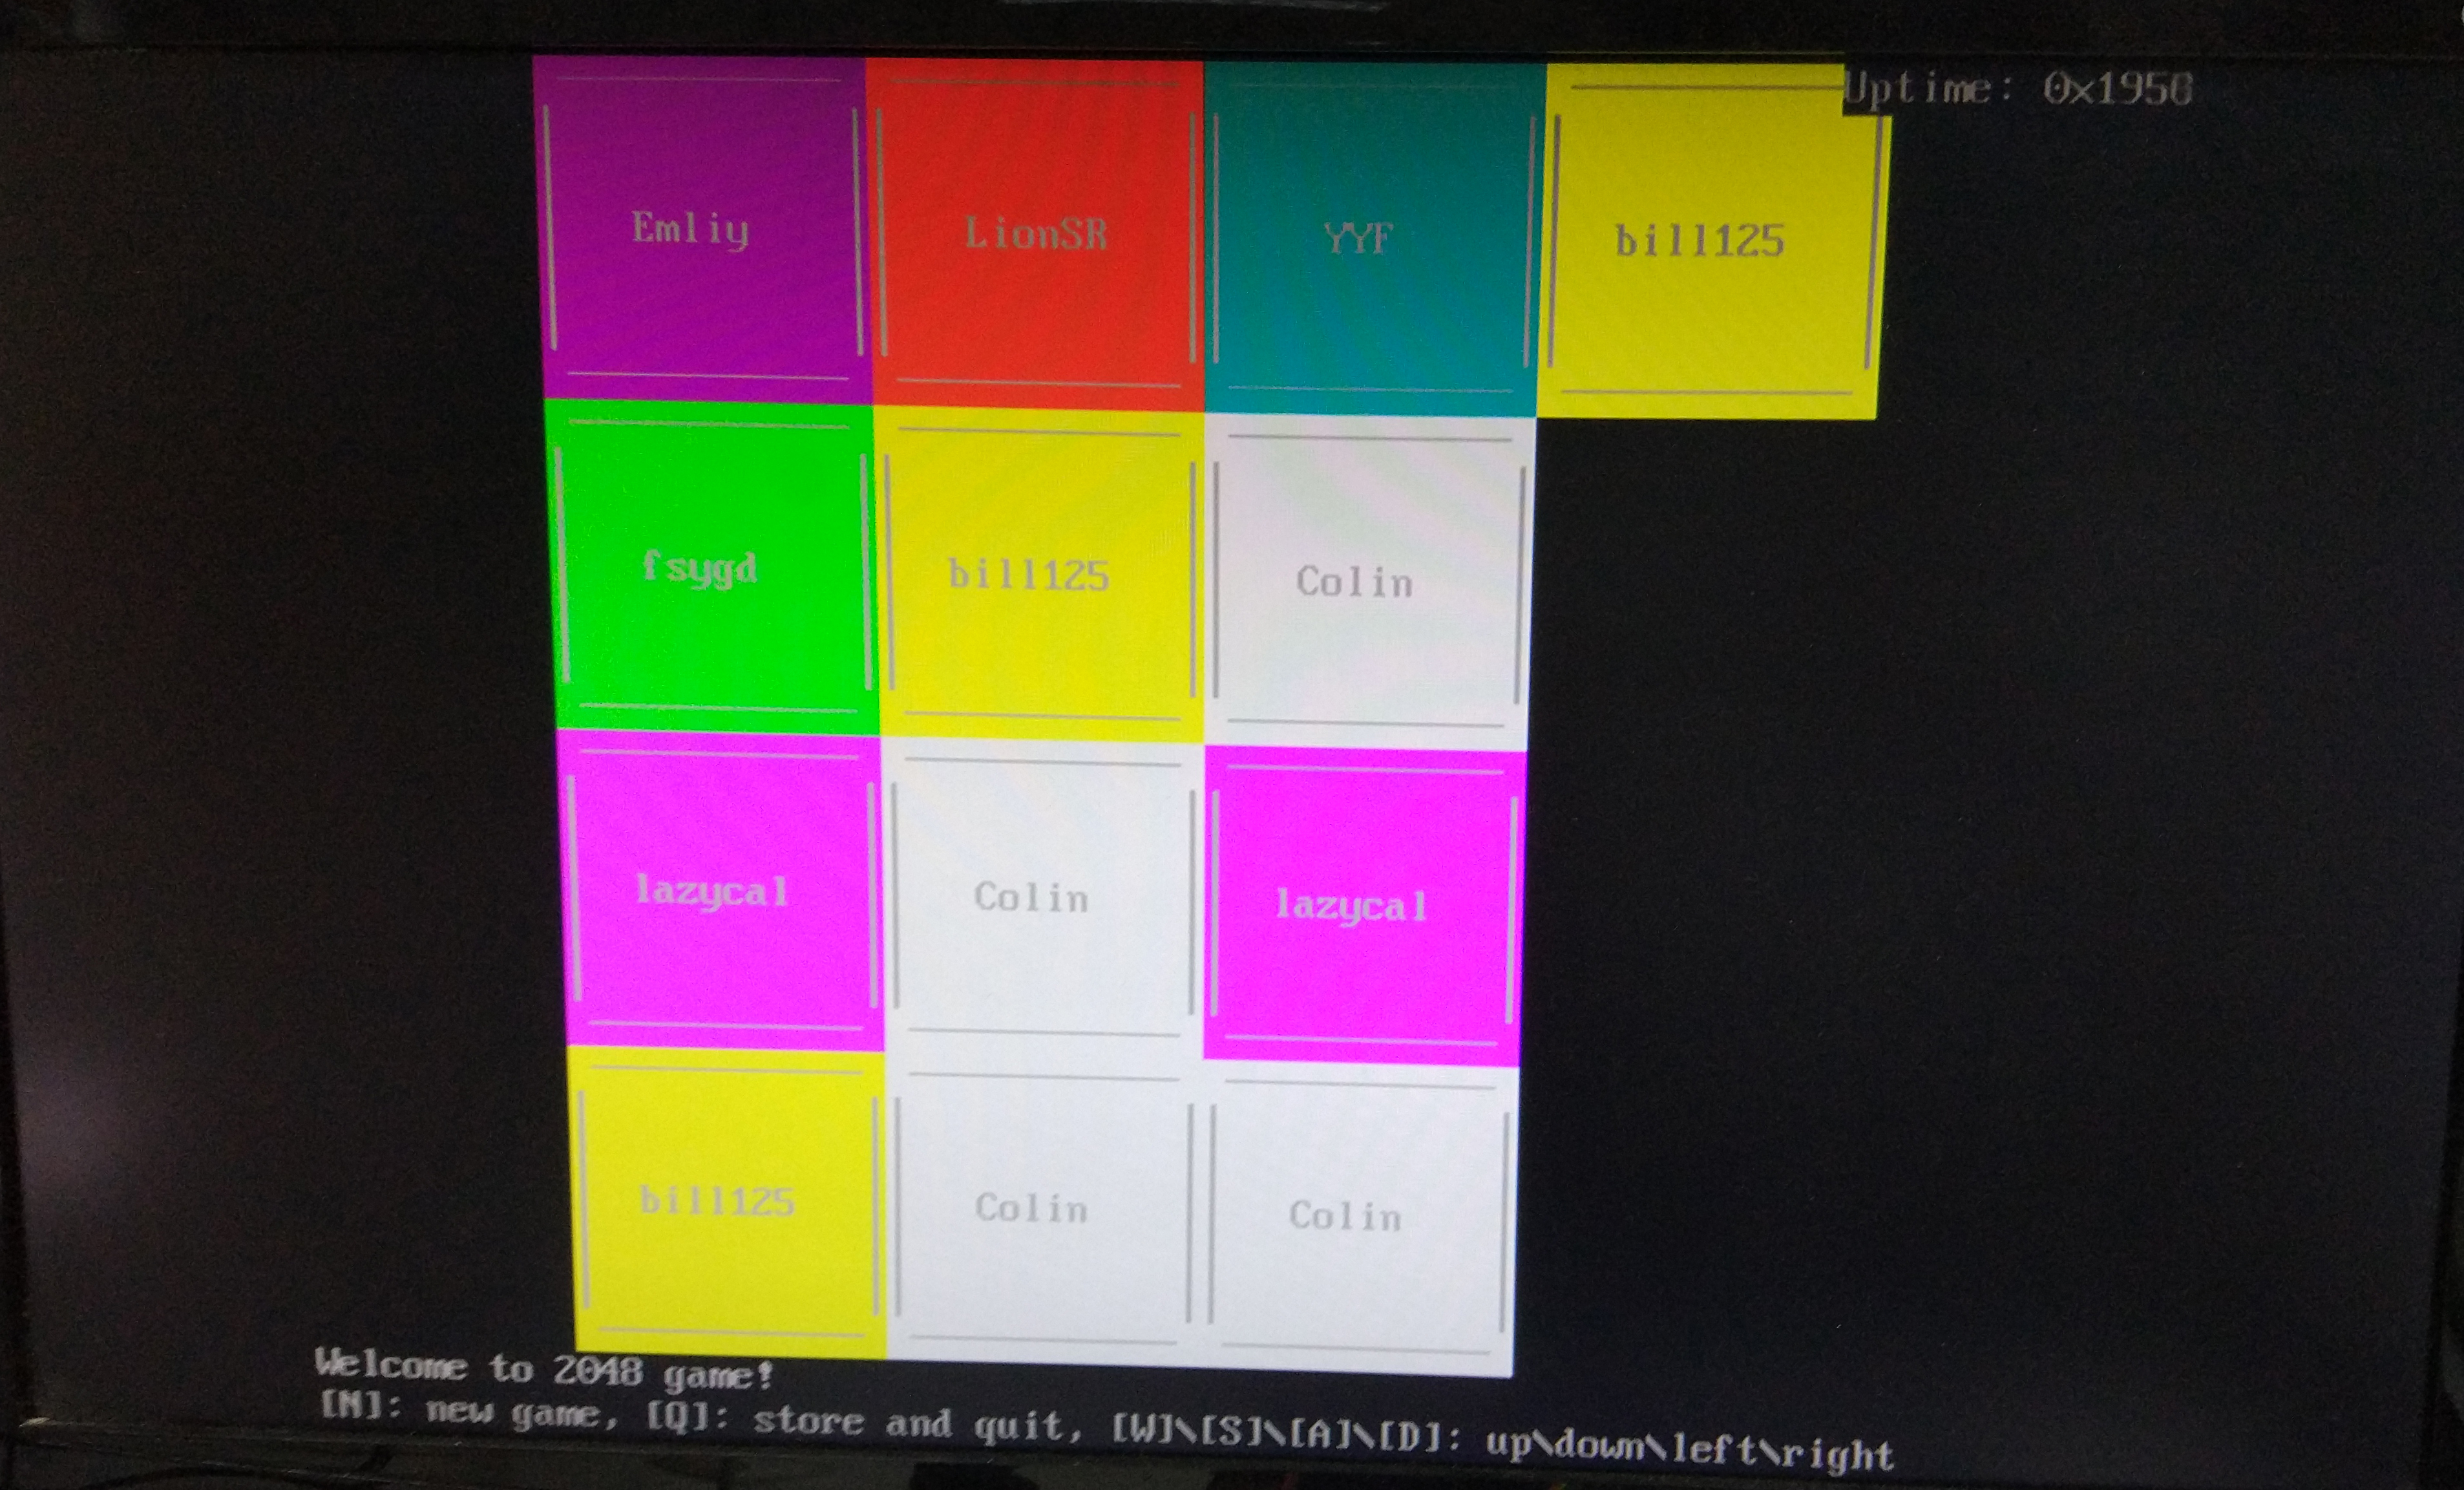
\includegraphics[width=0.8\textwidth]{2048.jpg}
			\caption{2048小游戏}
		\end{figure}
	\end{center}

2048是一款休闲益智游戏。玩家每次控制所有方块向同一个方向运动,两个种类相同的方块撞在一起之后合并成为更高级的块。每次操作之后会在空白的方格处随机生成一个最弱的块(Colin)。游戏胜利的条件是得到一个最强的叫做“lss”的方块,而如果16个格子全部填满并且相邻的格子都不相同,也就是无法移动的话,那么恭喜你,游戏结束了。此外,游戏胜利后并不会结束,两个“lss”方块合并后会有奇特效果。

在本系统中我们用汇编语言实现了一个上述游戏,支持随机开始新局面、从SD卡读盘、存盘到SD卡并退出等功能。具体来说一个游戏局面由16个方块对应的状态所构成,每次游戏开始时我们从SD卡加载游戏局面到内存。而在游戏过程中,程序将循环执行渲染局面、调用\texttt{getchar}阻塞地等待并读取用户输入、根据用户的输入执行相应的处理。

若用户输入的命令为\texttt{N},我们则随机生成一个包含若干最弱方块的新局面。其中,\texttt{getchar}中在等待PS/2控制器有新数据到来的时候维护一个计数器,可以用来产生伪随机数,熵由用户敲击键盘的间隔提供。

若用户输入的命令为\texttt{W}、\texttt{S}、\texttt{A}、\texttt{D},我们则根据用户的输入进行方块移动和合并的处理,之后再随机在空余位置生成最弱的方块。

若用户输入的命令为\texttt{ESC},我们则将当前游戏局面存盘到SD卡,再结束程序,返回shell。

而渲染一个局面时,我们需要显示欢迎语、游戏说明以及每一个方块的边框、文字,并进行着色。由于我们的显存存储的是80x30个ASCII字符及其对应的前景色和背景色,我们设计在游戏中每一个方块由$7\times14$个字符构成。其中每一种方块的背景色、文字均作为常量存储在内存中。在程序中我们只需循环计算每个方块的位置,并在显存中写入其所对应的$7\times14$个字符的内容和颜色即可。

值得一提的是,汇编程序不仅在编写上需要细心,而且由于我们的系统的简单性,缺乏行之有效的调试手段。在调试过程中,一个困扰我们许久的bug是程序分支指令的偏移量立即数长度有限,而我们的汇编器恰好没有对出问题的指令进行立即数溢出检查(现已补上),导致程序行为和预期不一致。

\subsection{BadApple!!动画播放} 
	\par TODO。

\subsection{BadApple!!的弹幕}

在本系统中,我们还实现了视频的弹幕功能,即在BadApple!!的动画播放过程中,用户可随时键入评论,并以换行符结束,用户键入的评论将随即从屏幕中飘过。

弹幕功能基于的是时钟中断,每隔5ms系统将触发一次时钟中断。若中断处理程序发现当前正在执行的是BadApple!!动画的播放程序,则会执行弹幕程序。弹幕程序主要执行两个功能:读取用户的键盘输入;当读取到换行符时将用户评论写入显存,并不断更新其显示位置以实现从屏幕中飘过的效果。

由于动画播放要求连续流畅且中断处理程序不支持被二次中断,故弹幕程序中的读取用户的键盘输入,以及循环显示评论都不能简单地使用阻塞的实现方式。具体来说我们用软件实现了一个状态机,将读取字符串操作变成了很多次中断来实现,每次先检查缓存区是否有新输入,如果有则调用\texttt{getchar}函数读取一个字符,并将其存入内存;若当前没有新输入,则直接结束中断。而在显示评论时,原来的循环刷新也要被改写成每次只刷新一次。因为被分成若干次调用,程序原来存放在寄存器中的计数器以及循环变量等都需要存放在内存中,并需记录程序当前执行到哪一个步骤,这些就是状态机的状态。

\subsection{内存转储}
	\par 这个程序相对比较简单。由于SD卡控制器支持DMA,所以这个程序只需要向SD卡控制器发送请求,把内存初始地址设为0、扇区数设为$64K * 2B / 512B = 256$,然后轮询方式等待SD卡操作完成即可。

\section{内存地址分配}

内存地址的分配需要软件和硬件配合来完成,我们的计算机系统中的内存分配如表\ref{mmap}所示。

\begin{table}[h]
\centering
\begin{tabular}{c|c|c}
\toprule[1.2pt]
\textbf{起始地址} & \textbf{结束地址} & \textbf{存储内容} \\
\midrule[1.2pt]
\texttt{0x0000} & \texttt{0x3FFF} & 内核代码 \\ \hline
\texttt{0x4000} & \texttt{0x7FFF} & 用户代码 \\ \hline
\texttt{0x8000} & \texttt{0xBEFF} & 数据段 \\ \hline
\texttt{0xBF00} & \texttt{0xBF00} & 串口控制器~数据寄存器 \\ \hline
\texttt{0xBF01} & \texttt{0xBF01} & 串口控制器~控制寄存器 \\ \hline
\texttt{0xBF02} & \texttt{0xDFFF} & 堆和栈 \\ \hline
\texttt{0xE000} & \texttt{0xFFFF} & IO内存映射区域 \\ \hline
\texttt{0xE000} & \texttt{0xE000} & GPIO控制器~数据寄存器 \\ \hline
\texttt{0xE001} & \texttt{0xE001} & GPIO控制器~方向寄存器 \\ \hline
\texttt{0xE002} & \texttt{0xE002} & PS/2控制器~数据寄存器 \\ \hline
\texttt{0xE003} & \texttt{0xE003} & PS/2控制器~控制寄存器 \\ \hline
\texttt{0xE004} & \texttt{0xE004} & 定时器~保留寄存器(暂未使用) \\ \hline
\texttt{0xE005} & \texttt{0xE005} & 定时器~控制寄存器 \\ \hline
\texttt{0xE006} & \texttt{0xE007} & 保留,未映射 \\ \hline
\texttt{0xE008} & \texttt{0xE008} & SD卡控制器~扇区号低16位 \\ \hline
\texttt{0xE009} & \texttt{0xE009} & SD卡控制器~扇区号高16位 \\ \hline
\texttt{0xE00A} & \texttt{0xE00A} & SD卡控制器~DMA内存地址低16位 \\ \hline
\texttt{0xE00B} & \texttt{0xE00B} & SD卡控制器~DMA内存地址高16位 \\ \hline
\texttt{0xE00C} & \texttt{0xE00C} & SD卡控制器~扇区数低16位 \\ \hline
\texttt{0xE00D} & \texttt{0xE00D} & SD卡控制器~扇区数高16位 \\ \hline
\texttt{0xE00E} & \texttt{0xE00E} & SD卡控制器~响应寄存器 \\ \hline
\texttt{0xE00F} & \texttt{0xE00F} & SD卡控制器~请求寄存器 \\ \hline
\texttt{0xE010} & \texttt{0xEFFB} & 保留,未映射 \\ \hline
\texttt{0xEFFC} & \texttt{0xEFFC} & 显示存储器~显存偏移地址低16位 \\ \hline
\texttt{0xEFFD} & \texttt{0xEFFD} & 显示存储器~显存偏移地址高16位 \\ \hline
\texttt{0xEFFE} & \texttt{0xEFFE} & 显示存储器~光标位置 \\ \hline
\texttt{0xEFFF} & \texttt{0xEFFF} & 显示存储器~光标闪烁计数器溢出值 \\ \hline
\texttt{0xF000} & \texttt{0xFFFF} & 显示存储器 \\
\bottomrule[1.2pt]
\end{tabular}
\caption{内存地址映射}
\label{mmap}
\end{table}

	\par 值得说明的是,我们把IO都被映射到了\texttt{0xE000}以上的地址,这是为了译码的时候方便(地址为\texttt{0xE000}以上的地址当且仅当其最高三位都为1)。

\chapter{未来可能的扩展空间}
	\par 进一步,我们还可以用汇编语言实现FAT16、ext2等文件系统,进而支持从外部存储器(SD卡)动态加载并运行程序。此外,还可以利用时钟中断实现上下文切换,进而实现多线程等现代操作系统所具有的特性。利用处理器对于外部中断的支持以及串口控制器和SD卡控制器的中断请求线,还可以实现异步IO,提高系统性能。此外,对于SD卡控制器,还可以加入更多的错误处理机制,而不是遇到错误就停机。

\chapter{参考文献}

$[1]$ 计算机硬件系统实验教程 

$[2] $ 自己动手写CPU 

$[3] $ CPU自制入门 

$[4] $ SD Specifications Part 1 Physical Layer Simplified Specification: \url{https://www.sdcard.org/downloads/pls/} 

$[5] $ How to Use MMC/SDC: \url{http://elm-chan.org/docs/mmc/mmc\_e.html} 

$[6] $ VGA Signal Timing: \url{http://tinyvga.com/vga-timing} 

$[7] $ Computer Organization and Design The Hardware/Software Interface Fifth Edition 

$[8] $ Computer Systems: A Programmer's Perspective Third Edition 

$[9] $ See MIPS Run Linux Second Edition 

$[10]$  FPGA设计实战演练(高级技巧篇) 

$[11]$  深入浅出玩转FPGA 第3版 

$[12]$  FPGA设计实战演练(逻辑篇) 

\end{document}
